\documentclass[a4,12pt]{scrartcl}

%Basic 
\usepackage[utf8]{inputenc}
\usepackage[ngerman]{babel}
\usepackage[T1]{fontenc}
\usepackage{float}
\usepackage[bottom = 3.50cm]{geometry}

%Titel Seite
\title{CLOUD INFRASTRUCTURE}
\subtitle{Lab-07}
\author{Giorgio Vincenti \and Samuel Krieg}
\date{\today}


%Kopf, Fusszeile
\usepackage{fancyhdr}
\pagestyle{fancy}
\lhead{ \begin{picture}(0,0) \put(0,0){
\includegraphics[width=3cm]{./pictures/hsrlogo.png}} \end{picture}}
\chead{}
\rhead{Seite \thepage}
\lfoot{Cloud Infrastructure \\Lab-07}
\cfoot{Giorgio Vincenti \and Samuel Krieg}
\rfoot{\today}
\renewcommand{\headrulewidth}{0.4pt}

%Bilder
\usepackage{graphicx}

%Tabellen
\usepackage{booktabs}

%Codesnippets
\usepackage{listings}
\lstset{language=bash} 

%Querformat für eine Seite
\usepackage{lscape}
\usepackage{rotating}
\usepackage{pdflscape}

%Temp
\usepackage{lipsum}



\begin{document}

\clearpage\maketitle
\thispagestyle{empty}
\tableofcontents
\newpage

\section{Anforderungen an ein modernes Datacenter}
\subsection{Herausforderungen}
Die Herausforderungen in einem moderem Datacenter bestehen darin die riesigen Datenmengen, die generiert werden, effizient und schnell verarbeiten zu können. Die Storages und Server Performance spielen dabei eine grosse rolle, jedoch bringt diese Performance nichts, wenn das Netzwerk nicht dementsprechend mit den Datenmengen effizient umgehen kann. Die grossen Datenmengen verlassen das Datacenter nicht, sondern fliessen von System zu System.

\subsubsection{Beispiele}
Hier einige Beispiele in der Praxis. \\

\noindent \textbf{VMotion:} Zum Beispiel bei Einsatz von Virtualisierung muss der Administrator in der Lage sein, VMs über das Netzwerk auf andere Hosts innerst kürzester Zeit verschieben können. \\

\noindent \textbf{Webserver:} Ein anderes Beispiel bezieht sich auf ein Webserver/Datenbank Modell. Der Webserver muss Daten der Datenbank abfragen und abholen ohne grossen Verzögerungen.\\

\noindent \textbf{Backup:} Ein weiteres Beispiel betrifft die Backups der Maschinen. Da fliessen ebenfalls grosse Datenmengen übers Netzwerk. Falls mehrere Server innerhalb eines gewissen Zeitraums gesichert werden müssen, muss die Netzwerkperformance stimmen, damit keine Engpässe auftreten. 

\subsection{Anforderungen}
Die Anforderungen an ein solches Datacenter sind sehr hoch. Da gibt es einiges zu beachten: 
\begin{itemize}
\item Sehr hohe Verfügbarkeit 
\item Mobilität von Applikationen, Systemen und Daten
\item Zugriffe auf Applikationen, Systemen und Daten 
\item Hohe Auto-Skalierbarkeit 
\item Genaue Abrechnungen auf benutzte Dienste 
\item Sicherheit 
\item Hohe Performance 
\item Abhängigkeit 
\item Autoprovisioning von Applikationen, Systemen und Daten
\end{itemize}

\subsection{Netzwerkarchitektur}
Die Netzwerkarchitektur spielt eine sehr grosse Rolle in einem Datacenter. Auch diese bringt grosse Anforderungen mitsich, damit das Beste aus der Infrastruktur rausgeholt werden kann. 
\begin{itemize}
\item Skalierbarkeit
\item Performance 
\item Hohen Datendurchsatz zwischen den Systemen
\item Elephant-flows fähig 
\item Managebar 
\end{itemize}

\section{TRILL}
\textbf{Tr}ansparent \textbf{I}nterconnection of \textbf{L}ots of \textbf{L}inks ist ein von der IETF festgelegten Standard.
\subsection{Funktion / Protokoll-Header}
\subsubsection{Funktion}
TRILL ist eine kombination von Layer 2 und Layer 3. Es ermöglicht auf Layer 2 zu routen und ersetzt Spanning Tree Protocol.
\subsubsection{Header}
\section{Trill - Teil 1}
\subsection{Function / Protocol header:} 
\begin{figure} [H]
	\begin{center}
	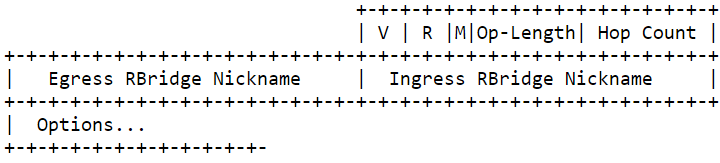
\includegraphics[width=0.80\textwidth]{./pictures/trill_header.png}
	\caption{\textbf{TRILL Header}}
	\label{x}
	\end{center}
\end{figure}
\begin{itemize}
\item V (Version): 2-bit unsigned integer.
\item R (Reserved): 2 bits.
\item R (Reserved): 2 bits.
\item Op-Length (Options Length): 5-bit unsigned integer.
\item Hop Count: 6-bit unsigned integer.
\item Egress RBridge Nickname: 16-bit identifier.
\item Ingress RBridge Nickname: 16-bit identifier.
\item Options: present if Op-Length is non-zero.
\end{itemize}

\subsection{Goal of TRILL:}
To uses Layer 3 routing techniques to create a large cloud of links which appear to IP nodes to be a single IP subnet. 

\subsection{Why was TRILL developed?}
\textbf{Tr}ansparent \textbf{I}nterconnection of \textbf{L}ots of \textbf{L}inks TRILL allows the ease of configuration of Ethernet while benefitting from the routing techniques provided at Layer 3.

\subsection{Where and how can TRILL be used?}
In datacenter for better migration of virtual machines. There will also be more bandwidth available for intensive applications like real-time communications and for the transport of storage traffic across the Ethernet network with FCoE and iSCSI.

\subsection{Is TRILL comparable to a traditional protocol?}It's a combination of traditional protocols (Ethernet, IP) and it's a bit like MPLS.
\subsection{What are the advantages and disadvantages of TRILL?}
TRILL make switches more cost-effective because it allows to load balance and to use more links in data center network designs.
Reduces Latency and improves overall network bandwidth utilization.
\subsection{Are there other modern technologies which are similar to TRILL} multichassis link aggregation or shortest path bridging
\subsection{How is TRILL configured in the LAB?}
\subsubsection{Trees}
\subsubsection{PacketFlow}
\subsubsection{MAC Learning} 
\newpage
\section{VXLAN - Teil 2}
\section{VXLAN with Arista switches}
\section{VXLAN Configuration}
\section{Research modern data center requirements}
Text jawoll ja

\end{document}
